\subsection{Reflection Effect}
\label{sect:reflect}

In this problem, you will create a reflection effect on an image.
The core of this transformation is this function:
\begin{quote}
\begin{lstlisting}
pixel_t[] reflect(pixel_t[] pixels, int width, int height);
\end{lstlisting}
\end{quote}
Your task here is to implement a function that takes as input an image
of size $w \times h$ and creates an output image four times as large.
The top right quadrant of the output image will contain the original
image, the top left will contain the input image reflected across the
$y$-axis, the bottom right will contain the input image reflected across
the $x$-axis, and the bottom left will contain the input image reflected
across both axes.  A sample image is shown in
Figure~\ref{fig:carnegie-reflect}.

If the original image has size $w \times h$, the returned image should
have size $2w \times 2h$. If the supplied array does not exactly match
the size given by the width and height, your function should abort with
a precondition failure when compiled and run with the \lstinline'-d' flag.

\begin{figure}
\centering
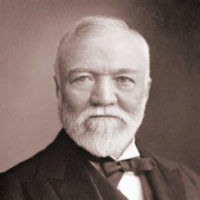
\includegraphics[scale=0.475]{\img/carnegie.png}
%\\[8em]
\quad\quad
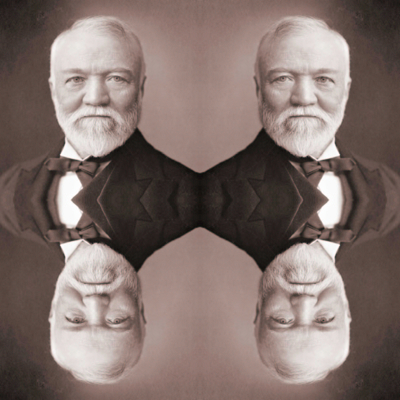
\includegraphics[scale=0.5]{\img/carnegie-reflect.png}
\caption{Original image (left); Image after ``reflection effect''}
\label{fig:carnegie-reflect}
\end{figure}

\vspace{0.1in}

\begin{task}[8]
\TAGS{array, correctness, safety, testing}
  Create a C0 file \lstinline'reflect.c0' implementing the function
  \lstinline'reflect'. You may include any auxiliary functions you need in the
  same file, but you should not include a \lstinline'main()' function.
\end{task}

You should look at \lstinline'README.txt' to see how to compile and run
this transformation using \lstinline'reflect-main.c0'. You are also
strongly encouraged to write some test cases for your
programs in \lstinline'images-test.c0'.


%%% Local Variables:
%%% mode: latex
%%% TeX-master: "main"
%%% End:
